\section{Explications techniques des fonctions et composants}
	\subsection{Pont}
	La figure~\ref{fig.pontseq} représente le diagramme de séquence du pont.
		\subsubsection{Fonctionnement}
		Le pont est composé de trois \emph{threads}. Le \code{main} démarre le module d’ethernet et attend qu’il soit connecté au routeur. Il démarre ensuite les deux \emph{threads} de communication. Finalement, il se met en veille et sert seulement au \emph{debug} par la suite. 

		Le premier \emph{thread} de communication est celui du Xbee. La librairie officielle de Digi pour Xbee est utilisée dans ce \emph{thread}. Le \emph{thread} traite les trames d’entrées et les places dans la \emph{mailbox} du \emph{thread} de communication Ethernet. Il écoute également de façon non bloquante sur sa propre \emph{mailbox} et envoie les messages aux Xbee correspondants lorsque nécessaire.

		Le deuxième \emph{thread} de communication est celui du Ethernet. Dans celui-ci, une librairie tierce HTTP est utilisée avec quelques modifications internes afin de transmettre et recevoir du JSON. Lorsque ce \emph{thread} reçoit un message du \emph{thread} de communication Xbee, il effectue une requête POST vers le serveur et attend une réponse (avec un \emph{timeout} de 1.5~secondes). Lorsque la requête revient, la réponse est transmise au \emph{thread} de communication Xbee. En cas d’erreur, un message d’erreur personnalisé est envoyé au \emph{thread} de communication Xbee. Tout est synchrone dans le \emph{thread} de communication Ethernet.

		Il est important de noter que le programme ne (dé)sérialise pas le JSON qu’il reçoit du serveur ou des Xbee. Cela est dû au fait qu’il manque de mémoire sur le MBED à cause de la bibliothèque Ethernet. Ainsi toutes les requêtes HTTP sont transmises au serveur sur le même \og endpoint \fg{} et les réponses sont transmises intégralement aux terminaux qui eux, s’occuperont de les traiter.
		
		\begin{figure}[p]
			\includegraphics[width=\textwidth]{Pictures/UML/reseauSequence}
			\caption{Diagramme de séquence du pont}
			\label{fig.pontseq}
		\end{figure}
	
	\subsection{Terminal de recharge}
	La figure~\ref{fig.rechseq} représente le diagramme de séquence du terminal de recharge.
		\subsubsection{Fonctionnement}
		Le terminal de recharge possède une architecture et un fonctionnement simple, basé sur une approche séquentielle. En effet, comme la réussite d’une recharge nécessite une série d'événements précis, le terminal est basé sur une machine à états finis (MEF) qui comporte 4~états. 

		Lorsque le terminal est mis sous tension, il s’ouvre dans l’état par défaut, soit l’état RFID. Le programme attend dans une fonction bloquante qu’un usager tape sa carte sur le lecteur RFID présent sur le devant du montage. Le numéro de la carte lue est gardé en mémoire.

		Une fois que le lecteur détecte une carte, le programme change l’état pour GET\_CLIENT\_INFO. Dans cet état, le programme utilise une librairie JSON pour construire un message recevable par le serveur et il l'envoie au pont à l’aide du module XBEE. Si tout s’est déroulé correctement, le programme reçoit une réponse du serveur avec le solde courant du client. Le solde est affiché sur l’écran présent sur le terminal. Le programme change alors l’état pour MONNAYEUR.

		Dans cet état, le programme alimente le monnayeur en courant, ce qui lui permet de recevoir des pièces de monnaie. Il est capable de prendre en entrée uniquement les pièces de 5, 10 et 25~cents, en plus des 1 et 2~dollars. Le programme reste actif à recevoir les pièces tant et aussi longtemps que l’utilisateur n’appuie pas sur le bouton présent sur le devant du montage. Le monnayeur envoie une série d’impulsions différentes selon la pièce déposée. C’est en comptant les fronts descendants que le programme est capable de savoir quelle pièce a été déposée. Une fois que l’utilisateur appuie sur le bouton, le programme change l’état pour SEND\_DATA et éteint l’alimentation du monnayeur, pour économiser de l’énergie. 

		Le dernier état de la MEF sert à ajouter le montant déposé au solde de l’utilisateur. Pour ce faire, le programme utilise encore la librairie JSON pour construire un message qu’il envoie via le module XBEE au serveur. Si l’envoi se passe bien, le programme reçoit une réponse du serveur avec le nouveau solde de l’utilisateur. Le programme affiche le nouveau solde à l’écran et retombe dans son état initial, en attente d’un nouvel utilisateur.
		
		\begin{figure}[p]
			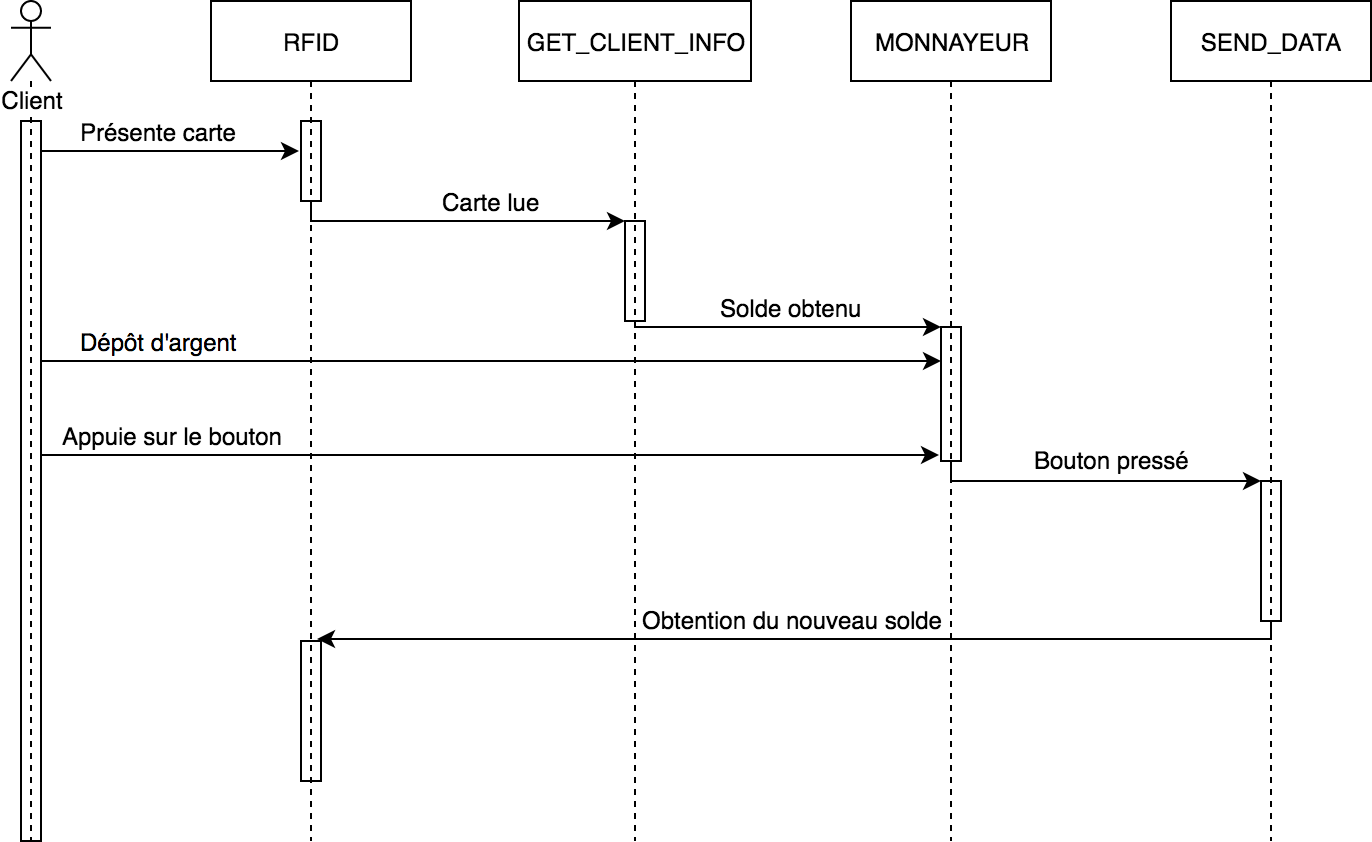
\includegraphics[width=\textwidth]{Pictures/UML/RechargeSequence}
			\caption{Diagramme de séquence du terminal de recharge}
			\label{fig.rechseq}
		\end{figure}
		
		\subsubsection{Protocole}
		Le terminal de recharge utilise deux types de messages JSON sur les quatre disponibles. Dans tous les cas, les messages des terminaux possèdent les champs \og id \fg{} (pour associer les réponses aux requêtes) et \og method \fg{} (afin d’indiquer au serveur la requête à effectuer). Il est également important de noter que tous les nombres sont des entiers et qu’il faut donc diviser par 100 pour tout ce qui est relié à l’argent.
		
			\paragraph{Ajout d'argent} Cette requête permet au terminal de recharge d’ajouter de l’argent au compte de l’utilisateur.
			%
			\begin{multicols}{2}	
				\begin{description}
					\item[Requête] \begin{lstlisting}
{
	"id": NOMBRE,
	"method": 3,
	"clientId": STRING, 
	"amount": NOMBRE
}
\end{lstlisting}
 % line break needed
					
					\item[Réponse] \begin{lstlisting}
{
	"id": NOMBRE,
	"balance": NOMBRE
}	
\end{lstlisting}
 % line break needed
					
				\end{description}
			\end{multicols}
			
			\paragraph{Solde} Cette requête permet au programme de récupérer le solde de l’utilisateur.
			%
			\begin{multicols}{2}
				\begin{description}
					\item[Requête] \begin{lstlisting}
{
	"id": NOMBRE,
	"method": 2,
	"clientId": STRING
}
\end{lstlisting}
 % line break needed

					\item[Réponse] \begin{lstlisting}
{
	"id": NOMBRE,
	"balance": NOMBRE
}
\end{lstlisting}
 % line break needed
					
				\end{description}
			\end{multicols}
			
	\clearpage
	\subsection{Terminal de paiement}
	La figure~\ref{fig.paieseq} représente le diagramme de séquence du terminal de paiement.
		\subsubsection{Fonctionnement}
		Le terminal de paiement partage quelques similarités avec le terminal de recharge. Son fonctionnement est très séquentiel pour la présente itération. Il est aussi basé sur une machine à états finis (MEF) à 5~états représentés dans une \og case/switch \fg{}.
		
		Le premier état au démarrage est GET\_MERCHANT\_ID. Dans cet état, le programme attend dans une boucle bloquante que l’utilisateur entre les 4~chiffres qui représentent son identifiant de marchand. Seuls les caractères numériques du claviers sont considérés. Une fois que cela est fait, le programme affiche une DEL verte et change l’état pour ENTER\_CART (qui est l’état par défaut pour le reste de l’exécution).

		Dans cet état, le marchand est invité à entrer une commande. Pour ce faire, une deuxième MEF a été introduite. Dans celle-ci, le marchand entre d’abord un nombre représentant la quantité à acheter. Il appuie ensuite sur \og F \fg{} et entre un deuxième nombre représentant le numéro du produit à acheter. Finalement, il peut appuyer sur \og E \fg{} pour ajouter un autre article en suivant la même procédure ou il peut appuyer sur «\og C \fg{} pour terminer la commande. Notons que tous les nombres ont un maximum de 4~chiffres pour les besoins du prototype et qu’une commande est limitée à 10~items. Lors de l’entrée de nombres, seuls les caractères numériques sont considérés.

		Lorsque la commande est complète, le programme revient dans la MEF principale à l’état GET\_CART\_TOTAL. Dans cet état, le terminal utilise la librairie JSON pour créer un message recevable par le serveur et l’envoie par Xbee au pont. Si tout va bien, il reçoit du serveur un message JSON qu’il décode pour avoir le total de la commande. Ce montant sera affiché sur l’écran pour le client.

		Le programme change alors l’état pour RFID. Dans ce dernier, le programme attend de façon bloquante que le client tape sa carte sur le lecteur RFID disposé sur le devant du terminal. Une fois que la carte est lue, le programme change pour l’état PAYMENT. Dans cet état, le programme utilise de nouveau la librairie JSON pour créer un message recevable par le serveur et l’envoie par Xbee au pont.  Si tout va bien, il reçoit du serveur un message JSON qu’il décode pour savoir si le paiement a été accepté et connaître le solde restant sur la carte. Une lumière s’affiche en conséquence (verte si tout est correct, jaune sinon) et le solde de la carte est affiché à l’utilisateur. Finalement, le programme revient dans l’état GET\_CART\_TOTAL.

		\begin{landscape}
			\begin{figure}[p]
				\includegraphics[width=1.5\textheight]{Pictures/UML/PaiementSequence}
				\caption{Diagramme de séquence du terminal de paiement}
				\label{fig.paieseq}
			\end{figure}			
		\end{landscape}


		\subsubsection{Protocole}
		Le terminal de paiement utilise deux autres types de messages JSON sur les quatre disponibles.
		
			\paragraph{Paiement}
			Afin d’effectuer un paiement, le programme envoie les items et les quantités associées à chaque item. Le \og clientId \fg{} est le numéro de la carte, et \og merchantId \fg{} est le numéro que le marchand entre au démarrage du terminal.
			%
			\begin{multicols}{2}	
				\begin{description}
					\item[Requête] \begin{lstlisting}
{
	"id": NOMBRE,
	"method": 1,
	"clientId": STRING,
	"merchantId": NOMBRE,
	"items": [11, 12, 14],
	"qty": [1, 5, 2]
}	
\end{lstlisting}
 % line break needed
					
					\vfill\null \columnbreak
					\item[Réponse] \begin{lstlisting}
{
	"id": NOMBRE,
	"status": False/True,
	"balance": NOMBRE
}	
\end{lstlisting}
 % line break needed
					
				\end{description}
			\end{multicols}

			\paragraph{Total}
			Cette méthode est semblable au paiement : elle permet de récupérer le prix de la commande selon les items que le client souhaite acheter.
			%
			\begin{multicols}{2}	
				\begin{description}
					\item[Requête] \begin{lstlisting}
{
	"id": NOMBRE,
	"method": 4,
	"merchantId": NOMBRE,
	"items": [11, 12, 14],
	"qty": [1, 5, 2]
}	
\end{lstlisting}
 % line break needed
					
					\vfill\null \columnbreak
					\item[Réponse] \begin{lstlisting}
{
	"id": NOMBRE
	"total": NOMBRE
}	
\end{lstlisting}
 % line break needed
					
				\end{description}
			\end{multicols}

	\subsection{Serveur et base de données}
		Un serveur \og node \fg{} assisté du langage javascript a été utilisé pour construire les fonctionnalités \og backend \fg{} de notre projet. Le serveur est constitué de deux parties principales : un service d’api et un site web. 
		
		\subsubsection{API}
		Le service d’api est du format REST. Il permet d’accéder, d’ajouter, de modifier ou de retirer des ressources de la base de données. Chacune de ces opérations est sans état. L’avantage d’utiliser un api REST est que toutes les plateformes intégrant une fonctionnalité de requête HTTP et de sérialisation json peuvent facilement accéder à nos services de manière standardisée et agnostique aux détails d’implémentation de notre serveur. Voici une liste des services de notre api : 
		%
		\begin{multicols}{3}
		\begin{itemize}
			\item Create Account
			\item Login Account
			\item Get Account
			\item List All Accounts
			\item Create Item
			\item Delete Item
			\item List Items
			\item Create Transaction
			\item List Transactions
		\end{itemize}
		\end{multicols}

		L’équipe a d’abord essayé d’utiliser les services ci-dessus avec le pont zigbee, cependant le micro-contrôleur du pont n’avait pas assez de mémoire pour sérialiser en JSON les informations reçues par ses n\oe{}uds, tel que mentionné précédemment. Cependant, les n\oe{}uds pouvaient le faire et le pont a donc été utilisé comme un relayeur des paquets JSON au serveur web. Toutefois, puisque le pont ne connaît pas le contenu des trames qu’il relaie, il ne peut envoyer ses requêtes qu’à un seul \og endpoint \fg{} de l’api REST. 

		Un \og endpoint \fg{} spécial nommé \og zigbee/bridge \fg{} a été créé pour désérialiser le JSON relayé par le pont zigbee et exécuter les actions nécessaires. Ce service comporte 4 fonctionnalités : 
		%
		\begin{itemize}
			\item Créer une transaction (débiter et créditer les bons comptes)
			\item Recevoir le montant restant sur un compte client
			\item Ajouter de l’argent à un compte
			\item Afficher le total pour un achat
		\end{itemize}

		
		\subsubsection{Site Web}
		Le site web est une interface qui permet aux marchands de voir leurs transactions effectuées, voir leurs produits, ajouter leurs produits et supprimer leurs produits. Les clients peuvent également accéder au site web pour voir leurs achats.
		
		\begin{figure}[p]
			\centering
			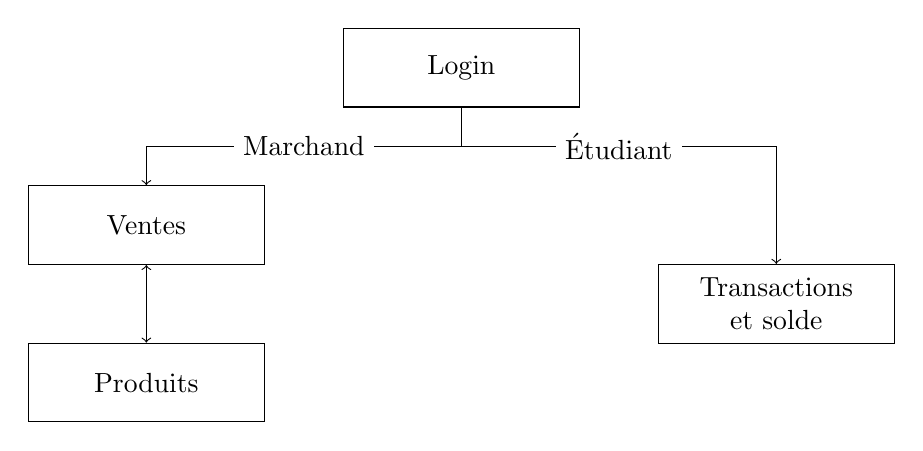
\begin{tikzpicture}[minimum height=1cm, minimum width=3cm, align=center]
	\node[draw] (prod) at (0,0) {Produits};
	\node[draw] (sales) at (0,2) {Ventes};
	\node[draw] (trans-solde) at (8,1) {Transactions \\ et solde};
	\node[draw] (login) at (4,4) {Login};
	%%%%%%%%%%%%%
	\draw[<->] (prod) -- (sales);
	\draw (login) -- (4,3);
	\draw (4,3) -- node[midway, fill=white, minimum size=0cm] {Marchand} (0,3);
	\draw (4,3) -- node[midway, fill=white, minimum size=0cm] {Étudiant} (8,3);
	\draw[->] (0,3) -- (sales);
	\draw[->] (8,3) -- (trans-solde);
\end{tikzpicture}
			\caption{Schéma des interactions avec le site web}
			\label{fig.schema}
		\end{figure}

		\begin{figure}[p]
			\fbox{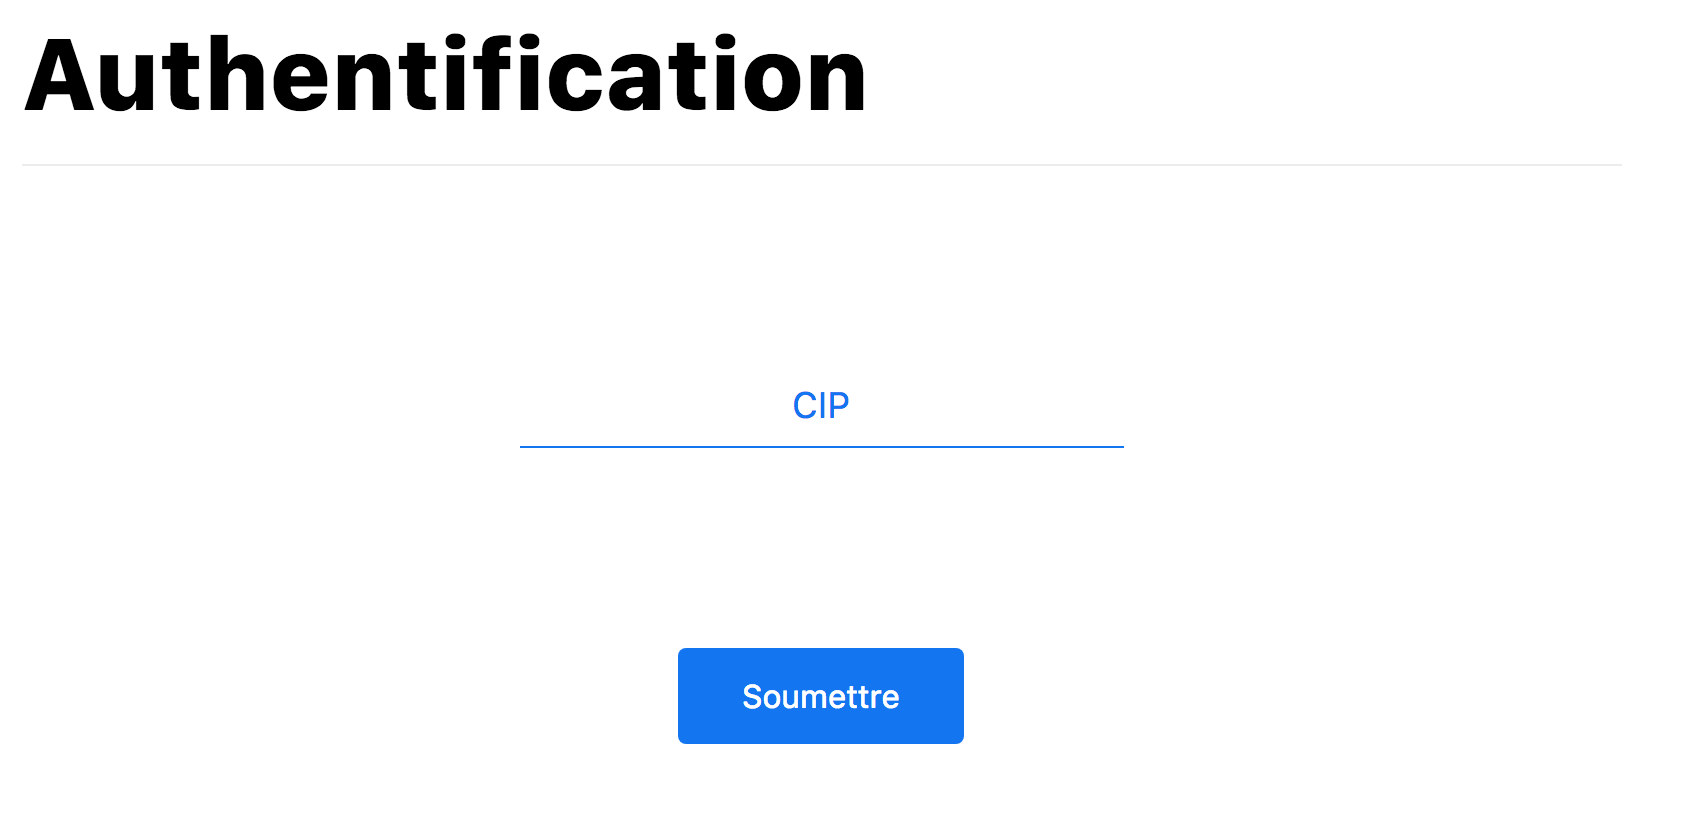
\includegraphics[width=\textwidth]{Pictures/web/authentification}}
			\caption{Fenêtre d’authentification du site web (login)}
			\label{fig.auth}
		\end{figure}

		\begin{figure}[p]
			\fbox{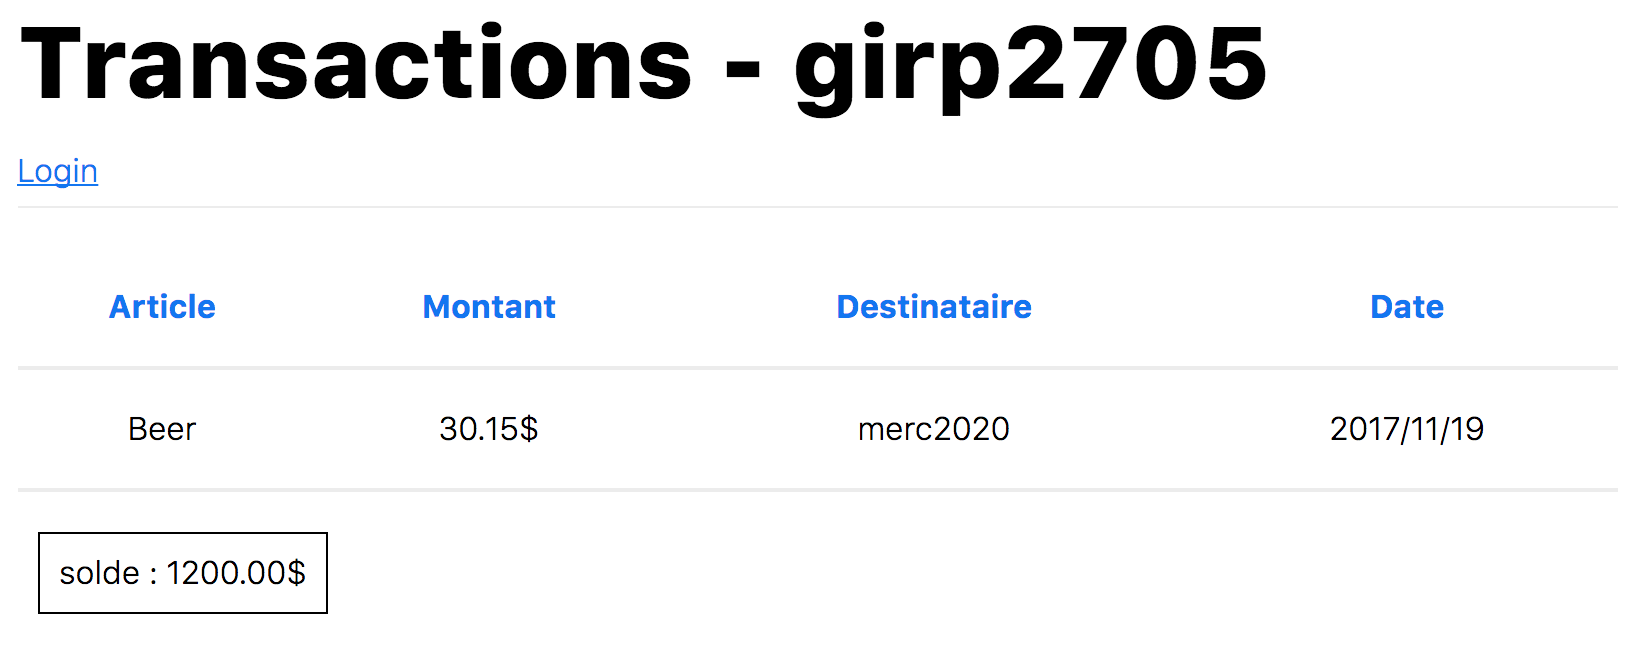
\includegraphics[width=\textwidth]{Pictures/web/transSoldeEtudiant}}
			\caption{Transactions et solde d’un étudiant}
			\label{fig.transEtudiant}
		\end{figure}
		
		\begin{figure}[p]
			\fbox{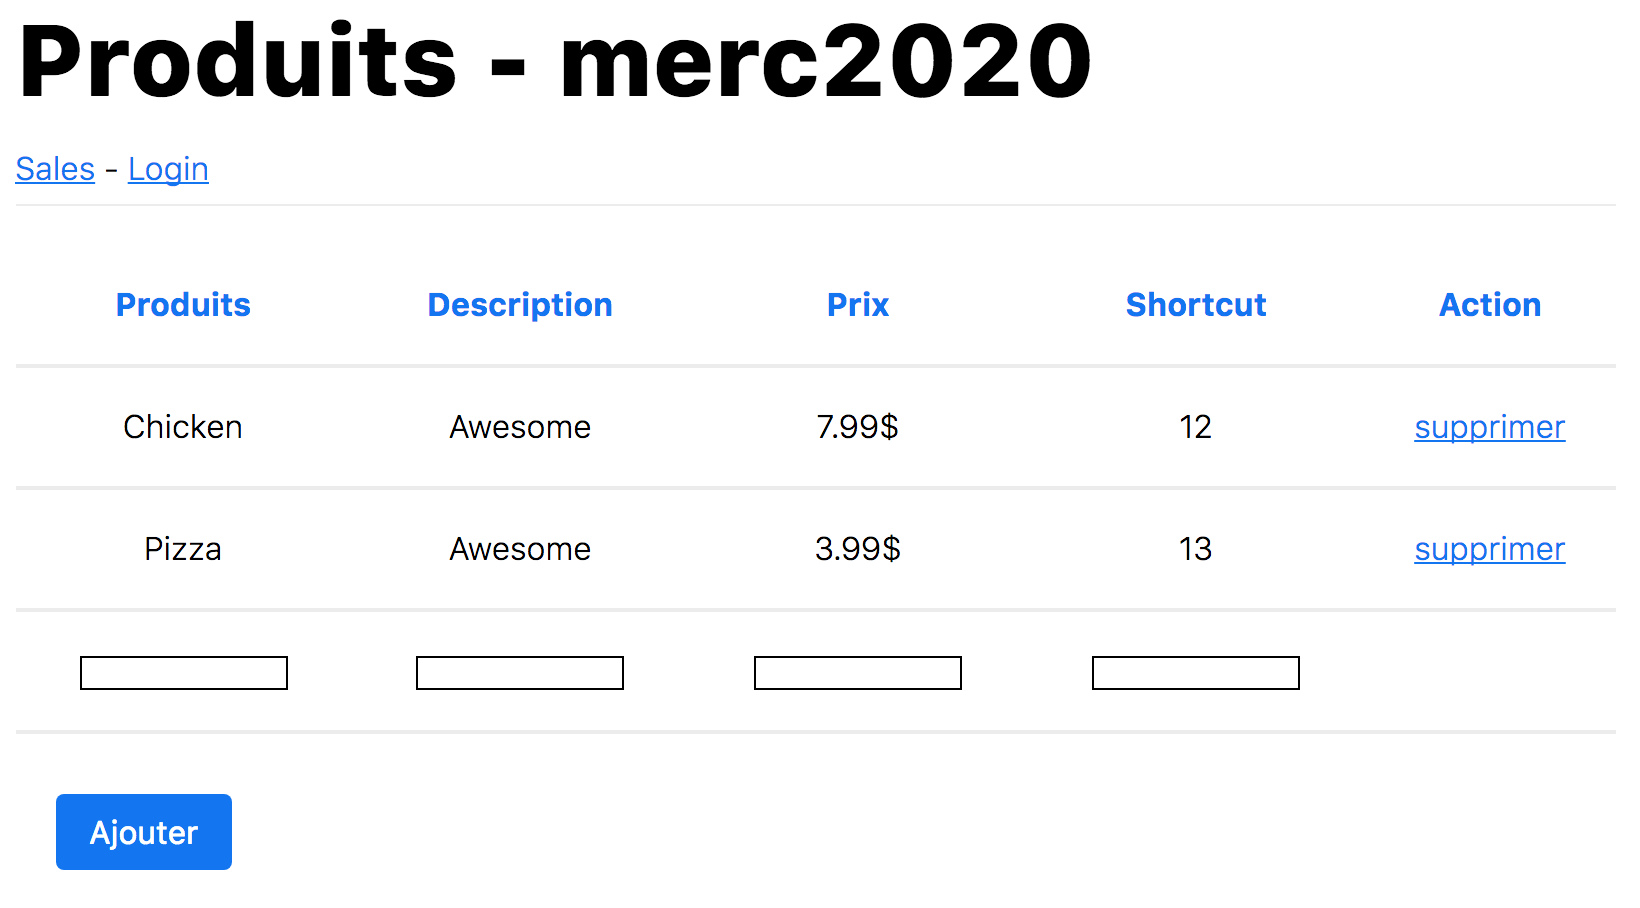
\includegraphics[width=\textwidth]{Pictures/web/produitsMarchand}}
			\caption{Liste des produits d’un marchand}
			\label{fig.prodMarchands}
		\end{figure}

		\begin{figure}[p]
			\fbox{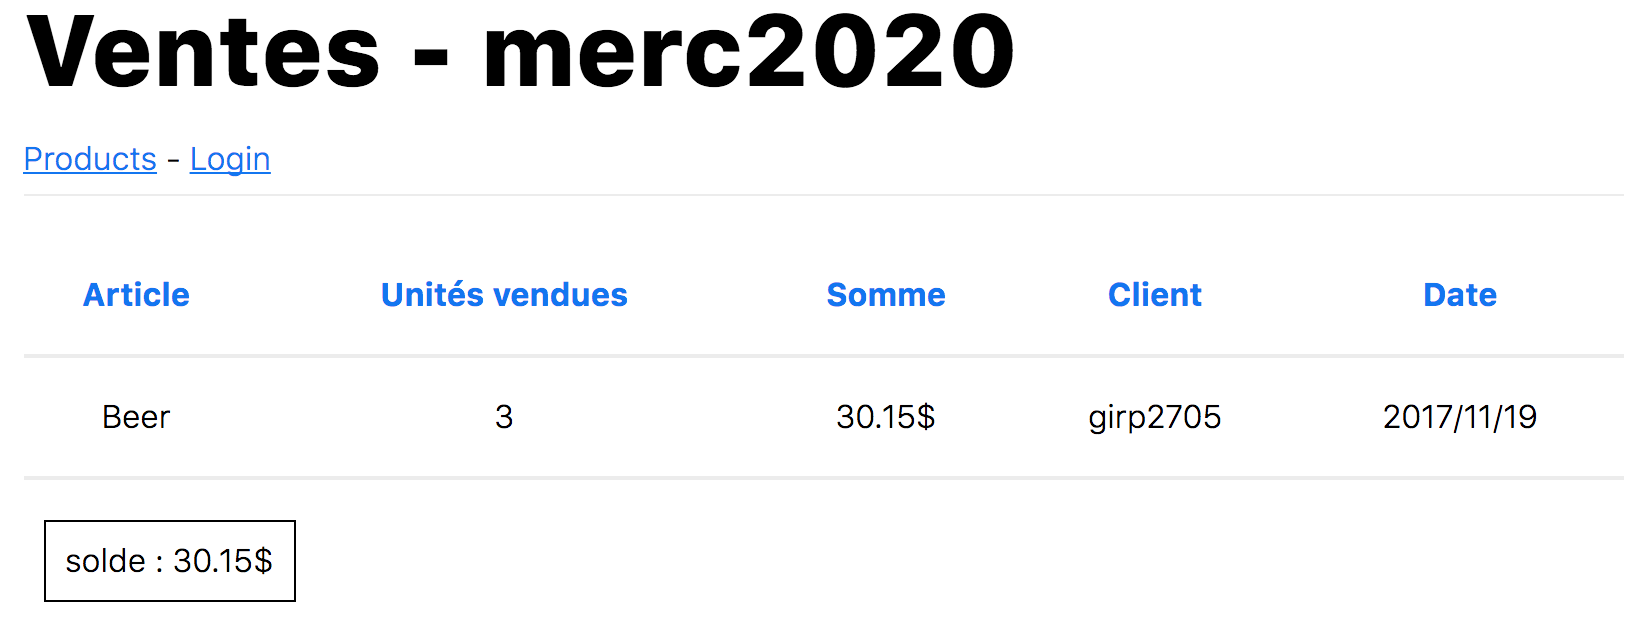
\includegraphics[width=\textwidth]{Pictures/web/ventesMarchand}}
			\caption{Ventes d’un marchand}
			\label{fig.ventesMarchands}
		\end{figure}

		Le site web a été créé sur le même serveur web que celui de l’api REST. Il utilise un modèle MVC. Il possède ses propres contrôleurs, routes et vues (\emph{views}), mais il partages ses modèles avec le service REST. Le \og rendering \fg{} de l’affichage se fait du côté serveur et des requêtes ajax sont utilisées pour rafraîchir les données automatiquement sans rafraîchissement de la page.
		
		\subsubsection{Postgres avec tables}
		Une base de données du format \emph{postgres} a été utilisée pour le projet, laquelle comporte 4 tables : 
		%
		\begin{itemize}
			\item Accounts
			\item Items
			\item Transactions
			\item LineItems
		\end{itemize}

		La table \og Accounts \fg{} comporte les comptes des clients et des marchands, leurs informations à propos de leur CIP, leurs cartes RFID, leur PIN et leur solde. La table \og Items \fg{}, fait la relation entre des items et un marchand qui les possède. La table \og LineItems \fg{} fait la relation entre des items, leur quantité et une transaction. La table \og Transactions \fg{} fait la relation entre un client et un marchand pour une transaction.

		Le plugin \og sequelize \fg{} a été utilisé pour faire nos modèles de la base de données en javascript et pour faire nos migrations de base de données ainsi que des \og seeds \fg{} pour la base de données.

		
		
		